%
%	Begrifflichkeiten
%

\pagebreak
\section{Targeting Background}

\onehalfspacing

\subsection{Targeted Advertising}

\subsubsection{Rationale}

Why do we need targeted advertising?

Let's start with the basics: Any advertising or marketing business has a vested interest to make their ads relevant, especially on the world wide web, where the user is, at least to a certain extent, anonymous. In its very basic, offline form, agencies would use context to place their ads; as an example you might see advertising for cars on busy roads or advertising for food near supermarkets.

In the online world, targeting users can be much more granular and automated, with the ideal outcome of showing an ad exactly at the right time and the right place (e.g. web site) for the user to see it, and with a need that it fulfills, have the user buy the product.

To achieve this, ad placement uses micro-targeting on the world wide web.

"Microtargeting is a marketing strategy that uses people’s data — about what they like, who they’re connected to, what their demographics are, what they’ve purchased, and more — to segment them into small groups for content targeting. It’s the reason that if you typically shop at Whole Foods, you may be served an advertisement for organic sunscreen during the Summer. And while it can help deliver content that is interesting and helpful to you, it also has a dark side — especially if it delivers information that’s inaccurate or biased and meant to sway your vote."\footnote{\textit{Ghosh, D. (2018)}: What is microtargeting? \cite{mozillaBlog}}

From a business point of view, micro targeting dramatically increases the relevance of the shown advertising and thus the likelihood of the user noticing it. Even if it does not lead to a sale right away, any product awareness helps and might lead to a sale in the future. 

Give the automated nature of ad placement on web pages, ads do not need to be shown in bulk, like in the offline world, but can be shown individually and with high relevance.

\subsubsection{Tracking}

To achieve this, it is necessary to gather more information on the interests of a particular user and follow their interests across the web; this mechanism is called tracking. Tracking as of today heavily relies on the use of cookies, small pieces of information stored in the users' browser, which we will explain in the next section.

Tracking can span web sites and companies - it is not limited to one company keeping a record of ones visits, currently it also includes the ability to analyze all visits on cooperating pages and show, for example, ads on Facebook based on your recent queries at Amazon. Technically this can be achieved through third-party cookies.

Third-party cookies are cookies set by another website than the one you're currently visiting and that can be later evaluated from the website.\footnote{See \textit{Cookie Script (2021)}: All you need to know about Third-Party Cookies \cite{mozillaBlog}}

Tracking through third-party cookies is under attack from multiple angles;\footnote{See \textit{Brinkmann, M. (2021)}: How Firefox new SmartBlock feature works \cite{mozillaBlog}} even \href{https://www.google.com/}{Google}, who invented it among various other tracking methods, will no longer support it in \href{https://www.google.com/chrome/}{Chrome} after 2023.\footnote{See \textit{Goel, V. (2021)}: An updated timeline for Privacy Sandbox milestones. \cite{sandboxDelay}}

\subsubsection{Cookies}

A cookie is a small piece of information that a server sends to the user's web browser for storage, and which it can request back at a later point in time.

Cookies can be used for session management, personalizing and tracking.\footnote{See \textit{Mozilla (2021)}: Using HTTP cookies \cite{usingCookies}}. For the purpose of this paper, we will focus solely on the tracking aspect, especially across sites, and not cover the more benign use cases for cookies, such as session management.

Cookies in itself are not malign and greatly support the user's experience across the web. however, they also show a persistent history of the user's activities.

Let's have a look at where cookies live on a user's browser. As an example, we will look at \href{https://www.mozilla.org/en-US/firefox/new/}{Firefox}, which stores its cookies in a \href{https://www.sqlite.org/index.html}{SQLite} database in the user's profile directory. Using \href{https://sqlitebrowser.org/}{DB Browser for SQLite}, we can examine the cookies:

\begin{figure}[H]
\centering
\caption {Cookies}
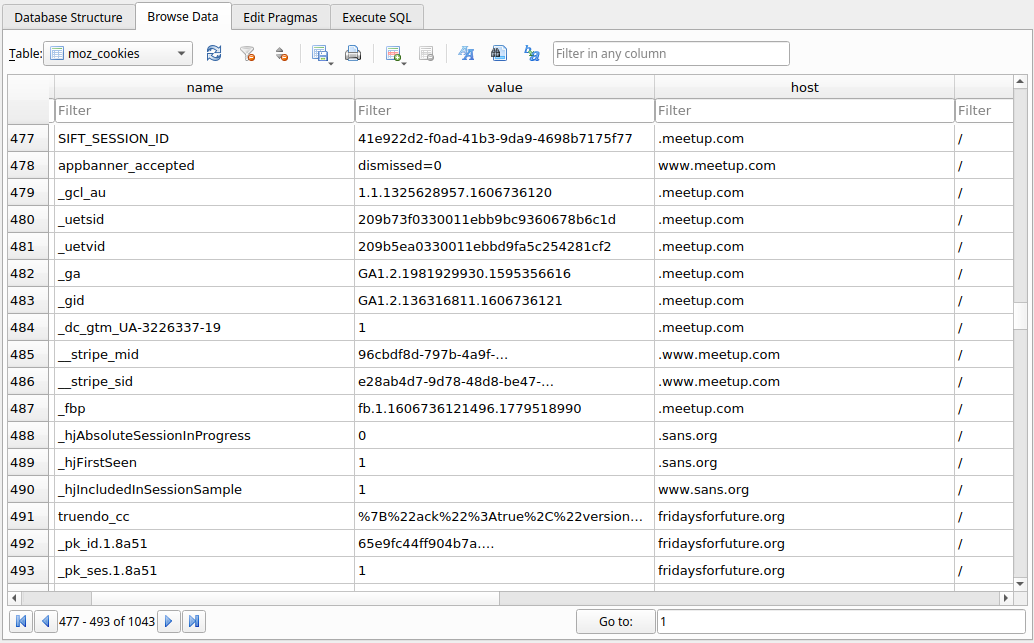
\includegraphics[width=\linewidth]{images/cookie-sqlite.png}
\label{fig:cookies}
\end{figure}

In its essence, cookies are a simple per-host key-value store in the browser; it's up to the web site to define which keys it wants to store. If a web site accesses it's own entries (as defined in the hosts column), that's called first-party data, or first-party cookies and could be used for session persistence, as seen in the first column.

If a web site accesses data from another site, that's when we're talking about third-party data, or third-party cookies which is used to track users on their visits across different web sites.

In addition to tracking in the web browser, there's also tracking in E-Mail\footnote{See \textit{Doffmann, Z. (2021)}: Why You Suddenly Need To Delete Gmail On Your iPhone \cite{deleteGmail}}, which we will not cover in this paper.

\subsection{Data Types}

\subsubsection{First Party}

Now that we have covered cookies as a mechanism to persist data in the user's browser, we need to look at the various classes of data. The definition for first party data is actually quite simple, it is data that we collect from our own sources.\footnote{See \textit{OnAudience (2019)}: What is first party data? \cite{firstParty}} Data could include information that we retrieve from our own cookies or from any information the user might have left on our website, for example by looking at an item.

In e-Commerce, a common use case would be to follow up on an abandoned sale, where the user looked at an item but did not put it into their shopping cart:

\begin{figure}[H]
\centering
\caption {Don't Wait}
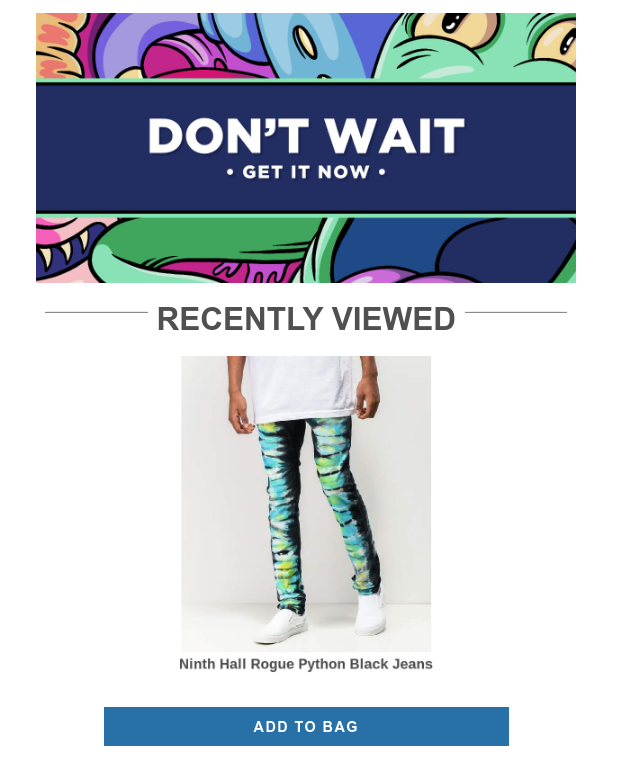
\includegraphics[width=\linewidth]{images/zumiez-dont-wait.png}
\label{fig:zumiez}
\end{figure}

This screenshot was taken from an E-Mail by \href{https://www.zumiez.com/}{Zumiez}; another example of clever use of first-party data are the regular notifications from \href{https://www.netflix.com/de-en/}{Netflix} to finish the season of a series you just started, or, as we will see below, the advertising on \href{https://smile.amazon.de/}{Amazon}.

% \begin{figure}[H]
% \centering
% \caption {Continue Watching}
% 
\includegraphics[width=\linewidth]{images/continue-boruto.png}
% \label{fig:boruto}
% \end{figure}

\subsubsection{Second Party}

The second class of data that we will look at is second party data. Simply speaking, second party data is another companies first party data.\footnote{See \textit{OnAudience (2019)}: What is first party data? \cite{firstParty}}

Assuming that two companies use the same identifier for their customers, for example the E-Mail address, one company could sell the shopping history on their site to another company, to enable them to advertise related products.

As we will see later in this paper, from a legal perspective, this is the most difficult setup to achieve as the company would need consent from its users to sell their data. It can be achieved though, for example within a conglomerate such as \href{https://www.facebook.com/}{Facebook}, \href{https://www.whatsapp.com/}{Whatsapp} and \href{https://www.instagram.com/}{Instagram}, where the platform users are explicitly asked to allow their data to be shared across all platforms.

If the proper agreements with the users are in place and the sharing is transparent, the use of second party data can be beneficial to both consumers and providers.

\subsubsection{Third Party}

The last class of data is third party data. It's defined as additional data that you buy from specialized sources on the web to enrich your own data.\footnote{See \textit{OnAudience (2019)}: What is first party data? \cite{firstParty}}

Third party data is inextricably linked to the use of third party cookies. As the user travels the web and leaves his traces in the cookies in his browser, data management platforms harvest this information, anonymize it, and create profiles from it.\footnote{See \textit{Shiffman, E. (2020)}: What is Third-Party Data? \cite{thirdParty}} These profiles are then sold and can be used to enrich ones own data.

With the impending demise of the tracking cookie, this aspect of the advertising business is in danger. As we progress in the paper, we will need to identify other ways to generate user profiles that we can use to display meaningful advertisement.

\subsection{Toolstack - Analytics}

\subsubsection{Google Analytics}

If we want to look at meaningful advertisement and successful placement, we first need to look at the tools that allow us to analyze traffic to our site and evaluate key performance indicators for our campaigns, such as Click-Through or Conversion rates.\footnote{See \textit{Romes, Y. (2020)}: 10 Inbound KPIs, die jetzt auch Personaler kennen sollten \cite{inboundKPI}}

\href{https://analytics.google.com/}{Google Analytics} is the most widely used tool for web traffic analysis and gives you, according to its website, all the necessary tools to analyze your web business data and gain insights into your campaign performances.

By looking at the data provided, we can gather deep insights into the visitors of our page and predict the performance of our posts.\footnote{See \textit{Frank, C. (2021)}: Web Traffic Analysis - Predicting Blog Post Performance \cite{previousBigdata}} We can also measure the effectiveness of our ad campaigns, which is a whole different topic. For the scope of this paper, we will solely focus on the data sources that we can use to place our campaigns.

\subsubsection{Open Source Analytics}

In addition to Google Analytics, there are a couple of other alternatives, some of which are \href{https://opensource.org/osd}{open source}. One example for open source analytics is \href{https://plausible.io/}{Plausible}, which I covered in a previous paper and which claims to be fully compliant to all major privacy legislation.\footnote{See \textit{Frank, C. (2020)}: Usefulness of open-source tools for web analytics in EMarketing \cite{previousPaper}} 

\begin{figure}[H]
\centering
\caption {Plausible}
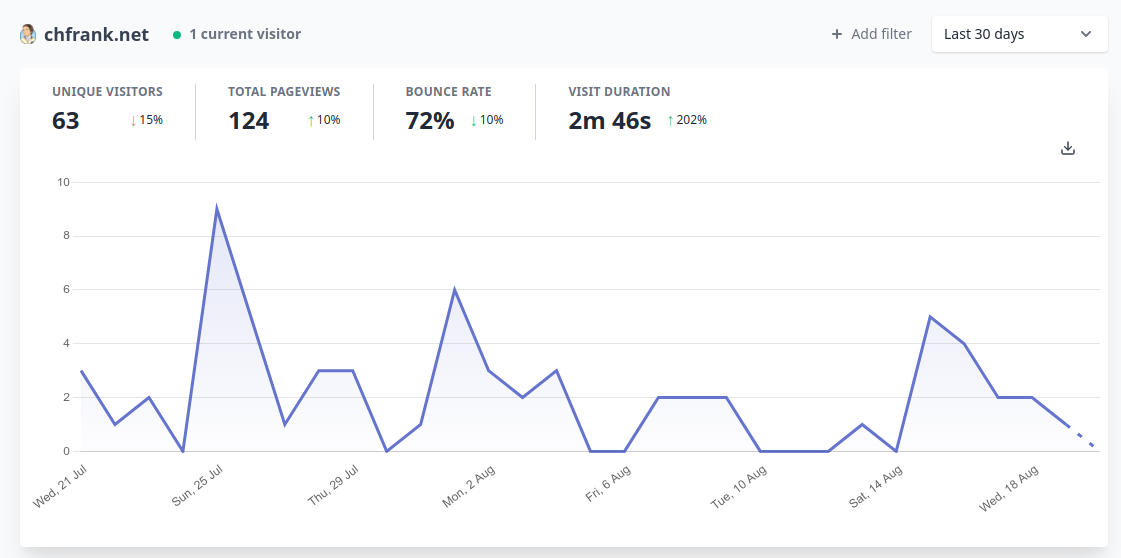
\includegraphics[width=\linewidth]{images/plausible.png}
\label{fig:plausible}
\end{figure}

\subsubsection{Yandex Metrica}

If you're reluctant to send data to the US for processing but are at the same time not invested in the open source side of software, \href{https://metrica.yandex.com/}{Yandex Metrica} is another commercial option for web page analytics, covering more than 8 million sites, according to their web page.

Metrica is part of the Yandex family of tools; Yandex is headquartered in Moscow, Russia and operates the biggest search engine there.

Yandex Metrica and Google Analytics are both operated by major search engine providers, which is not that surprising - in addition to crawling the web these search engines need to perform a lot of analytics themselves to put the most relevant search results on the first page. It makes a lot of sense to expose these analytics in some form to the end users.

How to optimize your placement on the search engine result page is again a whole different topic which we will not cover in this paper.

\subsection{Toolstack - Advertising}

\subsubsection{Google Ads}

Now that we have identified the data sources for successful advertising campaigns and the tools to measure the success, we need to look at the platforms that we can place our campaigns on. The biggest platform is \href{https://ads.google.com/home/}{Google Ads} and you can use it run campaigns on Google's search engine result pages and affiliates.

Ad placement on Google is based on search keywords and Google's knowledge of the user's profile; Google operate a bidding website where you place bids for certain terms and demographics to get your particular ad shown. Ad placement and the underlying algorithm is a science unto itself; recently Google has come under scrutiny from the regulators and in one case, agreed to the ruling and the fine.\footnote{See \textit{Burgess, M. (2021)}: France Cracked Down on Google’s Ad Tech \cite{googleAds}}

To target the most appropriate users for an ad, Google needs to have accurate information on the user itself and that's where data from third party cookies comes in.

It's important to differentiate between ad placement, which is a paid-for service, and search engine result page placement, which can be improved through Search Engine Optimization (SEO) techniques - even though both techniques are related to the Google search engine, they are not the same.

\subsubsection{Amazon Advertising}

The second biggest advertising platform is \href{https://advertising.amazon.com//}{Amazon Advertising}, a platform to place ads for your products on Amazon's pages and their affiliates.

The biggest difference to Google Ads is in that Amazon Advertising already has all the relevant data from their users through the Amazon shopping web site, it can almost operate entirely with first party data. Amazon Advertising also operates as a demand-side platform with selected partners, to increase the reach of the ads placed (second party data).

With ads focused on the Amazon shopping experience and consent from their users obtained on sign-up, Amazon's advertising business is not that much affected by the current discussion about third-party data.

\subsubsection{Facebook Advertising}

Last but not least we need to mention \href{https://www.facebook.com/business/ads}{Facebook Ads}, a platform to place ads on Facebook, Instagram, Messenger and the Audience Network.

Similar to Amazon, Facebook already has all the user profile data that it needs from its own platforms and has obtained consent during sign-up to share that data within its own family of businesses.\footnote{See \textit{WhatsApp (2021)}: What information does WhatsApp share with the Facebook Companies? \cite{whatsApp}}

Both companies, Amazon and Facebook, sit on a vast trove of invaluable first and second party data that they can freely use for their advertising business.

\subsection{Moving past cookies}

\subsubsection{Browser-based}

To continue with targeted advertising, even after the demise of the tracking cookie, new concepts and data sources are needed, some of which we will present in this paper. A common thread of all the new approaches is the attempt to make targeted advertising work, while at the same time maintaining the user's privacy; an umbrella term for these approaches is Privacy Preserving Advertising.\footnote{See \textit{Rescorla, E. (2021)}: The future of ads and privacy \cite{futureAds}}

The primary contender in the PPA space is \href{https://wicg.github.io/floc/}{Google FLoC}. The idea behing the federated learning of cohorts is actually quite simple, as it aims to expose the users' general browsing interest without exposing the browsing history, as it is the case today through the widespread use of third party cookies.

To achive this, Google proposes an algorithm to assign cohort ids to individual browsers, based on shared browsing habits. Then, instead of placing ads towards identifiable user profile data, ads would be placed against an anonymous cohort. 

The idea behind FLoC itself sounds quite reasonable, it is, however, under heavy fire from a privacy point of view.\footnote{See \textit{Rescorla, E. (2021)}: Privacy analysis of FLoC \cite{privacyFloc}} Among others, \href{https://www.eff.org/}{EFF}\footnote{Disclosure: I am a member and active supporter of EFF} has published a detailed analysis of FLoC's shortcomings in regards to privacy and why they believe that FLoC would be a terrible idea.\footnote{See \textit{Cyphers, B. (2021)}: Google’s FLoC Is a Terrible Idea \cite{terribleIdea}}

In a nutshell, all analysis questions the actual ability of FLoC to maintain the user's privacy and foresees a much broader tracking of users and their profiles than currently through the use of third party cookies.

\subsubsection{Data-based}

Another option would be to do away with third party data altogether and focus solely on first and second party data. One way to achieve this could be through data clean rooms, where independent contract processors would anonymously combine first party data of two or more companies. Having independent data trustees that vouch for anonymity would make sure that such data processing would most likely not run afoul of data protection regulations.\footnote{See \textit{Younger, M. (2019)}: The Three Hidden Technology Trends Behind Data Clean Rooms \cite{cleanRoom}}

Even though this approach sounds quite promising, such an independent infrastructure does not yet exist and no supra-national body has stepped up to create it.

\subsubsection{Identity-based}

Similar to FLoC are several other approaches to implement some kind of advertising ID, that would attempt to not violate the user's privacy rights but still allow for targeted advertising. The most prominent approach was Apple's ID for Advertising, which does not seem to be going anywhere for the time being.\footnote{See \textit{Ray, O. (2020)}: What is IDFA and Why Apple Killed it \cite{cleanRoom}}

Google also has an Advertising ID that supports ad personalization based on preference.\footnote{See \textit{Google (2021)}: Advertising ID \cite{advertisingId}} Similar to Apple's ID, Google offers an opt-out mechanism; if you opt out, only generic ads will be shown with much less relevance, and much less chance of a sale for the company placing the ad.

An industry consortium is release an open-source ID standard, UID2.\footnote{See \textit{The Trade Desk (2021)}: Unified ID Soltution 2.0 \cite{tradeDesk}} The basic premise is the same as for Google's or Apple's ID - the user is identified through a piece of personal information that is then encrypted and used as ID for the advertising profile. Unlike the approach from Apple and Google, however, the ID is not based on the device or the browser, but requires an active login. Quite elegantly this solves all issues around consent, but it remains to be seen how many users will login to an advertising network and share their preferences.

Microsoft is working together with Harvard on yet another standard\footnote{See \textit{Bird, S. (2020)}: Introducing the new differential privacy platform \cite{openDp}}, \href{https://opendp.org/}{OpenDP}, based on Differential Privacy.\footnote{See \textit{OpenDP (2020)}: What is Differential Privacy? \cite{diffPrivacy}} The conceptual idea behind differential privacy is quite interesting, but an analysis is out of scope for this paper.

\subsubsection{Content-based targeting}

Another quite promising approach is to forfeit user-based targeting altogether and concentrate solely on the browsing context. In 2020, the public radio in The Netherlands did this and went from targeted advertising to contextual advertising; quite surprisingly they saw their ad revenues grow.\footnote{See \textit{Edelman, G. (2020)}: Can Killing Cookies Save Journalism? \cite{killingCookies}} 

The system at \href{https://over.npo.nl/}{NPO} is a bidding system similar to Google Ads, however, ads are not placed based on a user profile but on the current context, i.e. a web page shown or a TV show watched. As far as the documentation shows, there's never any personally identifiable information being collected or transmitted and thus no issue with violating the user's privacy.

Abandoning the user profile in favor of context feels a bit like going back in time, but it does eliminate all privacy woes.

\subsection{Legal Framework}

As privacy comes into more and more focus, legislation is created all over the world, to better protect the user's privacy, eliminate unauthorized data collection and fight surveillance capitalism.\footnote{See \textit{Zuboff, S. (2020)}: You Are Now Remotely Controlled \cite{surveillance}} There's quite a number of legal frameworks that begin to govern tracking and advertising, so here's a list of the most common ones with links to the respective legal texts:

\begin{itemize}
 \item \href{https://gdpr-info.eu/}{GDPR} (General Data Protection Regulation)
 \item \href{https://www.datenschutz-grundverordnung.eu/}{DS-GVO} (Datenschutzgrundverordnung)
 \item \href{https://dsgvo-gesetz.de/bdsg/}{BDSG} (Bundesdateschutzgesetz)
 \item \href{https://dsgvo-gesetz.de/ttdsg/}{TTDSG} (Telekommunikations-Telemedien-Datenschutz-Gesetz (Entwurf ))
 \item \href{https://oag.ca.gov/privacy/ccpa}{CCPA} (California Consumer Privacy Act)
 \item \href{https://www.lgpdbrasil.com.br/}{LGPD} (Lei Geral de Proteção de Dados Pessoais)
 \item \href{https://popia.co.za/}{POPIA} (Protection of Personal Information Act)
 \item \href{https://ec.europa.eu/info/strategy/priorities-2019-2024/europe-fit-digital-age/digital-services-act-ensuring-safe-and-accountable-online-environment_en}{DSA} (Digital Services Act)
 \item \href{https://ec.europa.eu/info/strategy/priorities-2019-2024/europe-fit-digital-age/digital-markets-act-ensuring-fair-and-open-digital-markets_en}{DMA} (Digital Markets Act)
\end{itemize}

We cannot dive into the details on all these regulations; for the purpose this paper, we will assume that the reader is familiar with the content of the most important ones for Europe and Germany, the GDPR/DS-GVO and the BDSG, and will from here on solely focus on their impact and interpretation.

And as this is still an evolving situation, it's time to bring in the experts.
